\documentclass[14pt, fleqn, xcolor={dvipsnames, table}]{beamer}
\usepackage[T2A]{fontenc}
\usepackage[utf8]{inputenc}
\usepackage[english,russian]{babel}
\usepackage{amssymb,amsfonts,amsmath,mathtext}
\usepackage{cite,enumerate,float,indentfirst}
\usepackage{cancel}

\usepackage{tikz}                   
\usetikzlibrary{shadows}

% \usepackage{enumitem}
% \setitemize{label=\usebeamerfont*{itemize item}%
%   \usebeamercolor[fg]{itemize item}
%   \usebeamertemplate{itemize item}}

\graphicspath{{images/}}

\usetheme{Madrid}
\usecolortheme{seahorse}
\renewcommand{\CancelColor}{\color{red}}

\setbeamercolor{footline}{fg=Blue!50}
\setbeamertemplate{footline}{
  \leavevmode%
  \hbox{%
  \begin{beamercolorbox}[wd=.333333\paperwidth,ht=2.25ex,dp=1ex,center]{}%
    И. Кураленок, Н. Поваров, Яндекс
  \end{beamercolorbox}%
  \begin{beamercolorbox}[wd=.333333\paperwidth,ht=2.25ex,dp=1ex,center]{}%
    Санкт-Петербург, 2013
  \end{beamercolorbox}%
  \begin{beamercolorbox}[wd=.333333\paperwidth,ht=2.25ex,dp=1ex,right]{}%
  Стр. \insertframenumber{} из \inserttotalframenumber \hspace*{2ex}
  \end{beamercolorbox}}%
  \vskip0pt%
}
\newcommand\indentdisplays[1]{%
     \everydisplay{\addtolength\displayindent{#1}%
     \addtolength\displaywidth{-#1}}}
\newcommand{\itemi}{\item[\checkmark]}

\title{Линейные модели: SVM (продолжение). Collaborative filtering.\\\small{}}
\author[]{\small{%
И.~Куралёнок,
Н.~Поваров}}
\date{}

\begin{document}

\begin{frame}

\maketitle
\small
\begin{center}
\vspace{-60pt}
\normalsize {\color{red}Я}ндекс \\
\vspace{80pt}
\footnotesize СПб, 2013
\end{center}
\end{frame}

% Классные слайды http://www.cs.nyu.edu/~mohri/icml2011-tutorial/tutorial-icml2011-1.pdf
\section{SVM (продолжение)}
\begin{frame}{Что мы узнали в прошлый раз}
\small
\begin{itemize}
  \item Было бы классно найти такую плоскость, которая сильнее всего поделит на классы
  \item Если множества линейно разделимы, то надо минимизировать $\|w\|$
  \item Если перейти к дуальной задаче, зависимость от $x$ окажется только через скалярные произведения, которые мы можем ``организовать'' по своему разумению
  \item В дуальном решении условия очень просты и можно организовать безусловную оптимизацию заменой переменных
  \item Количество компонент оптимизации пропорционально квадрату количества точек, что много
\end{itemize}
\end{frame}

\subsection{SVM в случае неразделимых множеств} % из вики

\begin{frame}{Мягкие границы}
\begin{center}
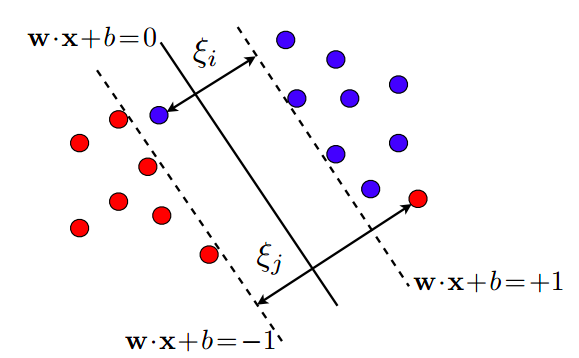
\includegraphics[height=0.4\textheight]{SoftMargins.png}
\end{center}
Перенесем точки-``нарушители'' на границу и добавим к целевой функции стоимость этого переноса:
$$\begin{array}{l}
\arg \min \|w\| + c\sum_i \xi_i \\
\left\{\begin{array}{l}
y_i(\beta^T x_i - b) + \xi_i \ge 1 \\
\xi_i \ge 0
\end{array}\right.
\end{array}$$
\end{frame}

\begin{frame}{Решение с мягкими границами}
\small
Прямая задача:
$$\begin{array}{ll}
\arg \min_{w,\xi,b} \max_{\lambda} & \|w\| \\
  & + c\sum_i \xi_i \\
  & - \sum_i \lambda_{i} \left(y_i (w x_i - b) + \xi_i - 1\right) \\
  & - \sum_i \lambda_{i+n} \xi_i \\
\lambda_i > 0
\end{array}$$

Дуальная задача (Wolfe):
$$
\begin{array}{l}  
\arg \max_{\lambda} \sum_{i=1}^m\lambda_i - \frac{1}{2}\sum_{i=1}^m\sum_{j=1}^m\lambda_i\lambda_j y_i y_j (x_i x_j) \\  

\left\{\begin{array}{ll}  
  0 \le \lambda_i \le c & \\
  \sum_{i=1}^m\lambda_i y_i = 0
  \end{array}   
\right.
\end{array}
$$
Где-то мы такое уже видели.
\end{frame}

\begin{frame}{Нелинейные решения в SVM (Ядра)}
Построим преобразование из исходного пространтсва в какое-то евклидово $\mathcal{H}$:
$$
\Phi: \mathbb{R}^n \to \mathcal{H}
$$
Тогда определим $(x_i, x_j) = (\Phi(x_i), \Phi(x_j))$. Что можно делать с ядрами \footnote{доказывается либо через определение, либо через теорему Мерцера}:
\begin{enumerate}
  \item линейно комбинировать
  \item умножать
  \item комбинировать с функцией, раскладываемой в Тейлора с неотрицательными коэффициентами (например $e^x$)
  \item etc.
\end{enumerate}
В задаче можно поставить цель подобрать оптимальное ядро с помощью подобных преобразований.
\end{frame}

\begin{frame}{Известные Ядра}
\small
\begin{description}
  \item[Полиномиальные] $K(x,x^{'}) = (x^Tx^{'} + c)^d$ 
  \item[Гауссово (radial basis)] $K(x,x^{'}) = e^{-\gamma \|x - x^{'}\|_2^2}$ 
  \item[Сигмойдное (``Нейронное'')] $K(x,x^{'}) = tanh(k_1 (x,x^{'}) + k_2)$ 
\end{description}
В этом случае решение будет выглядеть иначе:
$$
h(x) = sign \left(\sum_i \lambda_i y_i (K(x_i, x) + b)\right)
$$
Заметим, что можно выкинуть все точки в которых $\lambda_i = 0$ (это какие?).
\end{frame}

\subsection{Сведение SVM к линейной системе с регуляризацией} % из книжки

\begin{frame}{SVM и регуляризация}
\small
Вспомним как выглядит наша решающая функция (без ядер): $h(x) = sign(x^T w + b)$. Тогда проблему можно переформулировать так:
$$
\min \sum_i (1 - y_i h(x_i))_+ + \frac{\lambda}{2} \|w\|^2
$$
А это минимизация hinge loss с $l_2$ регуляризацией. Теперь тоже самое, но с ядрами, $h(x) = sign \left(\sum_i \lambda_i y_i (K(x_i, x) + b)\right)$:
$$
\min \sum_i (1 - y_i h(x_i))_+ + \frac{\lambda}{2} w^T K w
$$
где $K : k_{ij} = K(x_i, x_j)$. Нас никто не ограничивает hinge loss, можно все тоже самое, но с любым другим лосем!
\end{frame}

\begin{frame}{Kernel Ridge Regression}
\small
Если применима к любым функциям потерь, то почему не к $l_q$? Нормировка $b$ нам теперь не нужна, поэтому:
$$
h(x) = sign \left(\sum_i \lambda_i K(x_i, x)\right)
$$
Поигравшись в подстановку получим:
$$
\min_\lambda с \lambda^T\lambda - 2 \lambda y - \lambda^T K \lambda
$$
или
$$
\min_\lambda \lambda (K + cE) \lambda - 2\lambda^T y
$$
или
$$
\lambda = \left(K + с E\right)^-1y
$$
\end{frame}

%\subsection{Простая оптимизация SVM} % ? из головы /machinelearning.ru
\section{Построение мультиклассификатора} % best 10 years paper award ICML2010
\begin{frame}{Как построить мультиклассификатор?}
\begin{itemize}
  \item Выберем очки для каждого класса и сведем задачу к регрессии
  \item Один против всех в количестве $k$ штук
  \item Построим одновременно несколько классификаторов с условием их соотношения
  \item Есть еще идеи?
\end{itemize}
\end{frame}

\begin{frame}{Reducing multiclass to binary}
E.L.~Allwien, R.E.~Schapire, Y.~Singer предложили интересную альтернативу:
Введем модельную матрицу $\mathcal{M} \in \{-1,0,1\}^{k\times l}$. Для каждого столбца подберем функцию бинарной классификации, отделяющую $+1$ от $-1$.
Решим исходную задачу одним из двух способов:
$$
d_H(c, f(x), \mathcal{M}) = \sum_{s = 1}^l\left({1 - sign(m_{cs} f_s(x)) \over 2}\right)
$$
$$
d_L(c, f(x), \mathcal{M}) = \sum_{s = 1}^l L(m_{cs} f_s(x))
$$
Теперь вопрос свелся к тому как найти оптимальный $M$.
\end{frame}

\begin{frame}{Как найти оптимальный $M$}
Давайте строить последовательно: сначала первый столбец, потом второй etc. Введем меру:
$$\begin{array}{l}
\nu(f,\eta,x,y) = -\frac{1}{\eta} \log  \left(\frac{1}{l}\sum_{s=1}^{l} e^{-\eta m_{ys} f_s(x)}\right) \\
\eta = \sum_{t=1}^T \alpha_t \\
f_s(x) = \sum_{t=1}^T \alpha_t h_t(x, s) \\
\\
M_{f,\eta}(x,y) = \frac{1}{2}\left(\nu(f,\eta, x, y) - \max_{r\ne y}\nu(f,\eta,x,r)\right)
\end{array}$$
\end{frame}

\section{Collaborative filtering}

\subsection{Пример} % переработать http://habrahabr.ru/company/surfingbird/blog/139022/ на Сифона/Бороду
\subsection{Постановка задачи} % wiki

\subsection{Случай, когда матрица полная} % Воронцов, лекция в ВШЭ http://www.machinelearning.ru/wiki/images/e/e5/Voron-2008-11-10-cf.pdf
\subsection{Разреженные матрицы: решение факторизацией} %  из головы
\subsection{Простое SVD разложение}  % Гантмахер
\subsection{Известные регуляризации} % Мучать Гулина
\subsection{Factorization machines} % Статья http://www.ismll.uni-hildesheim.de/pub/pdfs/Rendle2010FM.pdf
\end{document}
